\section{Entraînement}
Nous avons donc deux réseaux, un actor et un critic.
Notre objectif est de faire apprendre le MDP(Markovian Decision Process) au critic, et d’optimiser la policy de l’actor de façon à maximiser le nombre de récompenses qu’il peut obtenir dans ce MDP.
Il existe plusieurs méthodes permettant de faire converger ces réseaux vers des politiques optimales. 
La plupart de ces méthodes permettent de définir la policy optimal d’un agent pour un champ d’actions discrétisé.

\begin{figure}[H]
    \centering
    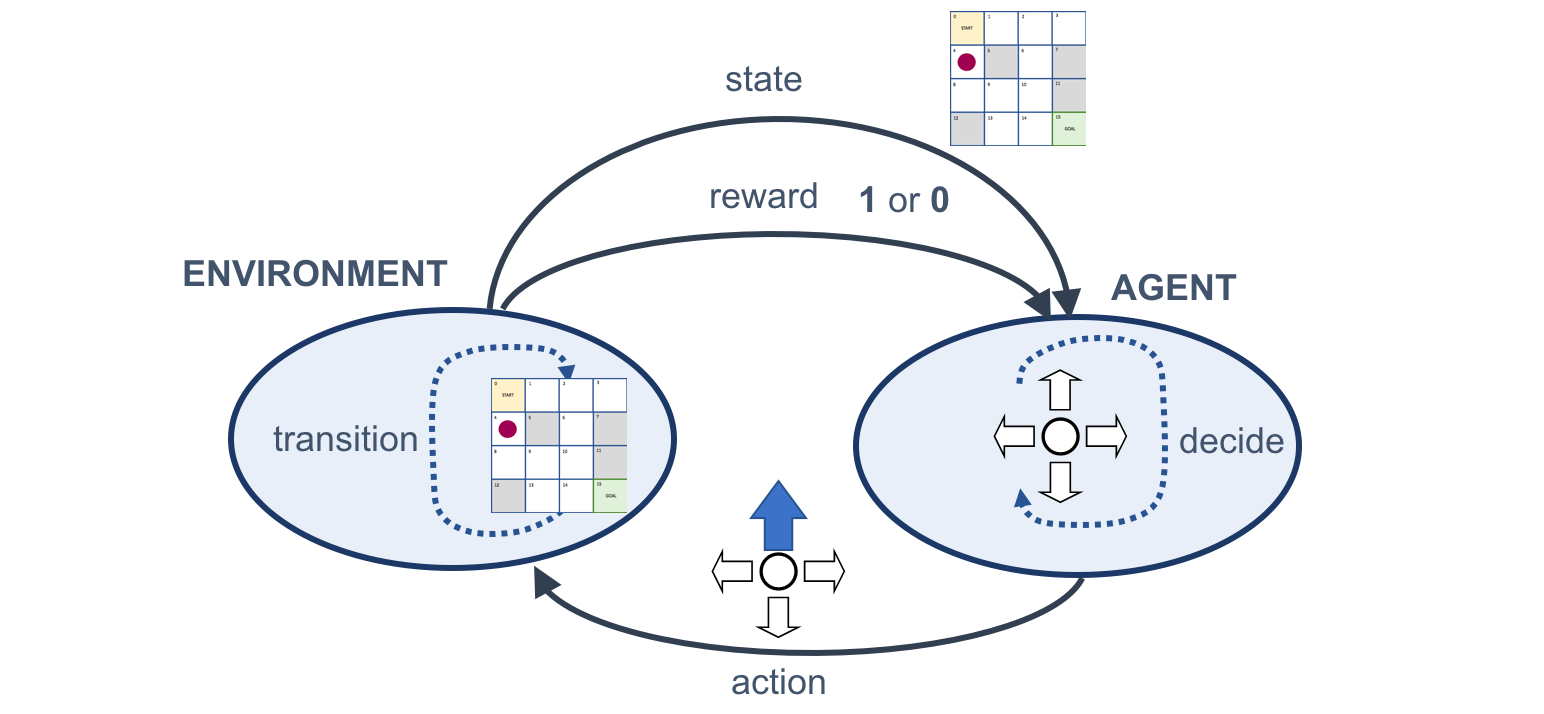
\includegraphics[width=0.5\textwidth]{./image_RL/image38.png}
    \caption{ Renforcement champ d’action discrétisé. }
\end{figure}

Pour résoudre ce problème, nous voulons que notre agent soit capable de définir la commande sur les trois axes XYZ. Une première approche peut être de discrétiser les valeurs que peut prendre le robot pour s’orienter de façon à copier les méthodes plus conventionnelles.
Nous voulions absolument avoir un champ de commandes continu sur les 3 axes de façon à trouver la policy optimal. Ce qui n’aurait pas été le cas avec une discrétisation.
Nous avons donc dû utiliser un algorithme spécifique appelé DDPG.

\subsection{DDPG (Deep Deterministic Policy Gradient)}
Le Deep Deterministic Policy Gradient (DDPG) est un algorithme off-policy model-free pour l'apprentissage d'actions continues.
Il est expliqué de façon exhaustive dans l’aticle[4].
Il combine les idées de DPG (Deterministic Policy Gradient) et de DQN (Deep Q-Network). 

\begin{figure}[H]
    \centering
    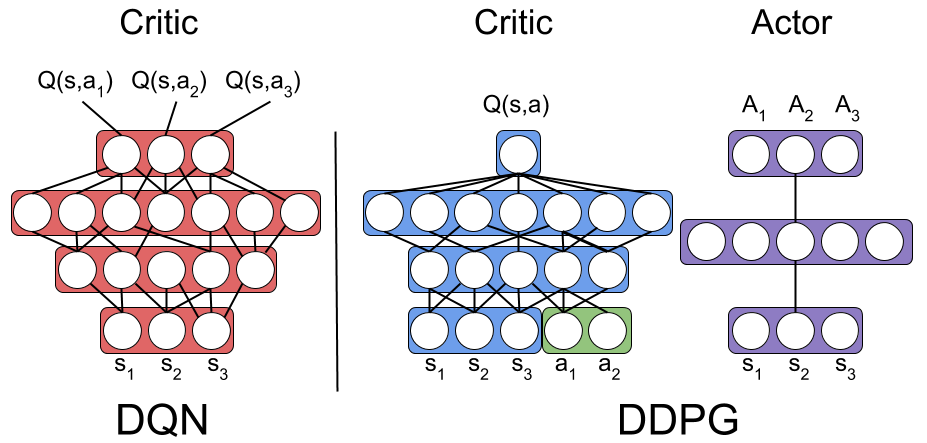
\includegraphics[width=0.5\textwidth]{./image_RL/image10.png}
    \caption{  DQN vs DDPG  }
\end{figure}

\textbf{Off-policy:}

Entraîner un réseau off-policy traduit le fait qu’on entraîne l’agent avec des actions qu’il n’a pas réalisé dans l’environnement. C’est en fait l’agent qui apprend le comportement d’un autre agent dans l’environnement.
Ici la frontière est difficile à percevoir. 
On considère que l’on entraîne en off-policy du fait que l’on déphase les phases d’apprentissage et d’exploration avec deux agents.
En effet, on va utiliser un agent pour explorer l’environnement et un agent target pour entraîner le premier agent.
Cette méthode est utilisée dans d’autres algorithmes car elle permet de stabiliser l’apprentissage.
Dans l’algorithme de DDPG elle est essentielle dans la mesure où l’agent n’est entraîné que par le critic.
En effet, il faut déphaser les phases d’entraînement du critic et de l’actor, sinon le critic n’entraîne pas l’actor comme il faut et l’actor n’explore pas l’environnement de façon à apprendre une politique intéressante. Il s’agit d’un cercle vicieux duquel il ne peut pas sortir.

\textbf{Model-free:}
Le terme model-free traduit simplement que l’on ne connaît pas le MDP puisque c’est le critic qui va nous permettre de l’estimer.


\begin{figure}[H]
    \centering
    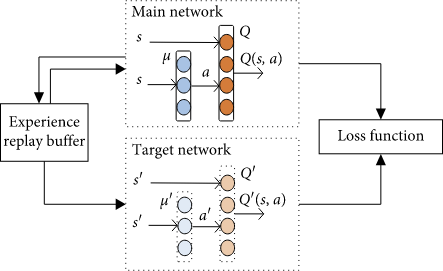
\includegraphics[width=0.5\textwidth]{./image_RL/image6.png}
    \caption{  Graphique de fonctionnement du DDPG  }
\end{figure}

Comme on peut le voir, le target network va servir à entraîner le main network qui lui fait l’exploration. Ensuite le target network va mettre à jour ces poids dans la même direction que les poids du main network mais très lentement. Ce processus permet au réseau d’apprendre en agile. On peut prendre la métaphore de l’éclaireur. Le main network part en éclaireur et test différentes policy qu’il peut critiquer grâce à la vision du target network.
Petit à petit le target network met à jour sa vision de l’environnement et sa policy en fonction de ce qu’à découvert le main network.
Cela retarde l’entraînement mais permet de le stabiliser. En effet, l’un des problèmes les plus récurent en deep reinforcement learning est lorsque l’actor trouve une policy qui ne permettra plus au critic d’apprendre et comme le critic apprend à l’acteur, on tombe dans un cercle vicieux.
On pourrait penser qu’il suffit de diminuer la taille du learning rate de façon à ralentir l’entraînement. Ça serait une erreur.
En effet, le fait d’utiliser un target network permet de découvrir énormément de policy possible et ensuite de sélectionner celle qui lui on permit d’obtenir le meilleur nombre de reward.
